\documentclass[a4paper,14pt]{extreport} % формат документа

\usepackage{amsmath}
\usepackage{cmap} % поиск в ПДФ
\usepackage[T2A]{fontenc} % кодировка
\usepackage[utf8]{inputenc} % кодировка исходного текста
\usepackage[english,russian]{babel} % локализация и переносы
\usepackage[left = 2cm, right = 1cm, top = 2cm, bottom = 2 cm]{geometry} % поля
\usepackage{listings}
\usepackage{graphicx} % для вставки рисунков
\usepackage{amsmath}
\usepackage{float}
\usepackage{multirow}
\graphicspath{{pictures/}}
\DeclareGraphicsExtensions{.pdf,.png,.jpg}
\newcommand{\anonsection}[1]{\section*{#1}\addcontentsline{toc}{section}{#1}}

\lstset{ %
	language=Lisp,                % Язык программирования 
	numbers=left,                   % С какой стороны нумеровать          
	frame=single,                    % Добавить рамку
}

\begin{document}
\begin{titlepage}

    \begin{table}[H]
        \centering
        \footnotesize
        \begin{tabular}{cc}
            \multirow{8}{*}{
\includegraphics[scale=0.35]{bmstu.jpg}}
            & \\
            & \\
            & \textbf{Министерство науки и высшего образования Российской Федерации} \\
            & \textbf{Федеральное государственное бюджетное образовательное учреждение} \\
            & \textbf{высшего образования} \\
            & \textbf{<<Московский государственный технический} \\
            & \textbf{университет имени Н.Э. Баумана>>} \\
            & \textbf{(МГТУ им. Н.Э. Баумана)} \\
        \end{tabular}
    \end{table}

    \vspace{-2.5cm}

    \begin{flushleft}
        \rule[-1cm]{\textwidth}{3pt}
        \rule{\textwidth}{1pt}
    \end{flushleft}

    \begin{flushleft}
        \small
        ФАКУЛЬТЕТ
        \underline{<<Информатика и системы управления>>\ \ \ \ \ \ \ 
        \ \ \ \ \ \ \ \ \ \ \ \ \ \ \ \ \ \ \ \ \ \ \ \ \ \ \ \ \ \ \ 
    \ \ \ \ \ \ \ \ \ \ \ \ \ \ \ } \\
        КАФЕДРА
        \underline{<<Программное обеспечение ЭВМ и
        информационные технологии>>
        \ \ \ \ \ \ \ \ \ \ \ \ \ \ \ \ \ \ \ \ }
    \end{flushleft}

    \vspace{2cm}

    \begin{center}
        \textbf{Лабораторная работа № 1} \\
        \vspace{0.5cm}
    \end{center}

    \vspace{4cm}

    \begin{flushleft}
        \begin{tabular}{ll}
            \textbf{Дисциплина} & Моделирование.  \\
            \textbf{Тема} & Генераторы псевдослучайных чисел.  \\
            \\
            \textbf{Студент} & Сиденко А.Г. \\
            \textbf{Группа} & ИУ7-73Б \\
            \textbf{Оценка (баллы)} & \\
            \textbf{Преподаватель} & Рудаков И.В.   \\
        \end{tabular}
    \end{flushleft}

    \vspace{4cm}

   \begin{center}
        Москва, 2020 г.
    \end{center}

\end{titlepage}

\begin{enumerate}

\item \textbf{Условие. }

Изучить и реализовать генератор псевдослучайных чисел: программный и табличный. Получаем числа 1-разрядные, 2-разрядные, 3-разрядные. Сравниваем по критерию. Вывод.  

\item \textbf{Теория. }

\textbf{Табличные генераторы} в качестве источника случайных чисел используют специальные таблицы, содержащие некоррелированные, то есть никак не зависящие друг от друга, цифры.

С помощью  \textbf{программных генераторов} получаются псевдослучайные числа, то есть каждое последующее сгенерированное число зависит от предыдущего. 

 \textbf{Критерий случайности. }
 
Для определения равномерности распределения воспользуемся частотным тестом, который позволяет определить сколько чисел попало в интервал $(m-\sigma, m+\sigma)$, где $m$ -- математическое ожидание последовательности случайных чисел, $\sigma$ -- среднеквадратичное отклонение. 
 
За ожидаемое количество случайных чисел примем отношение длины этого интервала ко всему интервалу, на котором генерируются случайные числа. 

Полученным количеством будет отношение чисел попавших в этот интервал к общему числу случайных чисел.  

\item \textbf{Полученные результаты. }

\begin{figure}[H]\center
	\begin{tabular}{cc}
		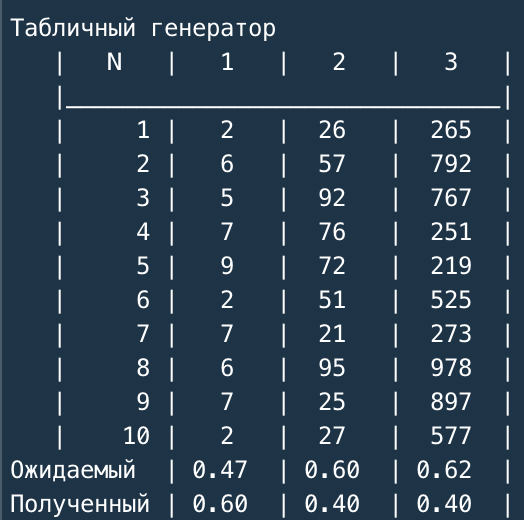
\includegraphics[width=80mm]{extable1} & 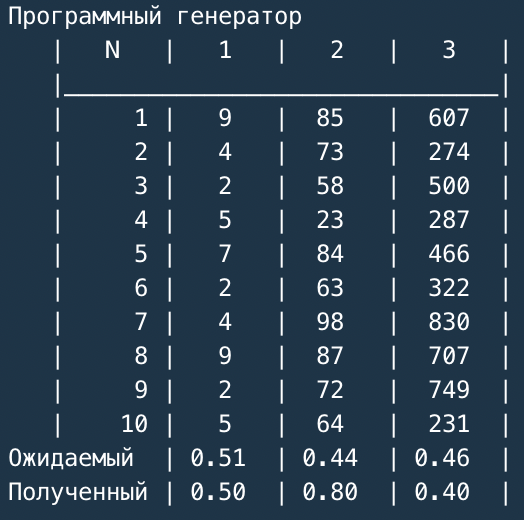
\includegraphics[width=80mm]{exprog1} \\
		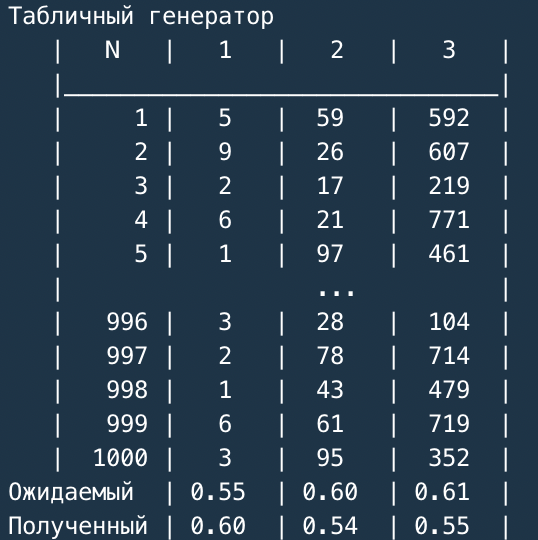
\includegraphics[width=80mm]{extable2} & 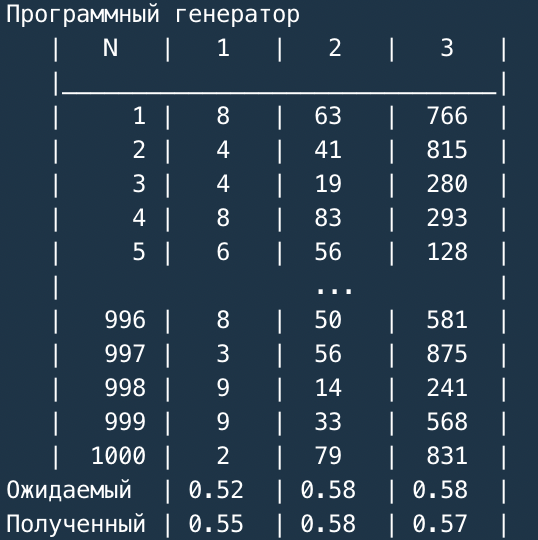
\includegraphics[width=80mm]{exprog2} 
	\end{tabular}
	\\ Рис. 1 -- Примеры работы
\end{figure}

\item \textbf{Вывод. }

Таким образом из результатов видно, что чем больше количество генерируемых случайных чисел тем равномернее они распределены. Также исходя из полученных значений критерия, программный генератор генерирует более равномерную последовательность, в сравнении с табличным.  

\end{enumerate}
\end{document}